\documentclass[12pt]{article}

\usepackage[13643]{easymcm}  % Team control number
\usepackage{longtable}
\usepackage{booktabs}
\usepackage{algorithm}
\usepackage{algpseudocode}

\newcommand{\toB}[1]{\color{blue}#1\color{black}}

\problem{A}  % Problem number

\title{Paper Name}  % Title

\begin{document}

\begin{abstract}

	Some random text
	
\end{abstract}

\maketitle
\tableofcontents

\section{Introduction}

	\subsection{Problem Background}
		
		
		
	\subsection{Problem Restatement}
	
		some random text

\section{Dandelion Spread Model}

	\subsection{Assumptions and Justifications}
	
		\begin{enumerate}
			
			\item \textbf{The dandelion is located at the midpoint of an edge of a square field, which has dimensions of 100m$\times$100m (1 hectare).  When seeds are blown out of the field, they are neglected.}
			\vspace{-0.125in}
			\begin{description}
				\item[Justification:] The problem states that the dandelion is adjacent to the field.  Thus, we consider the dandelion to be located on the edge of the field.  Furthermore, we limit our consideration within the field.  Seeds that land outside the field are considered to be negligible, possibly due to a river or forest that borders the field.
			\end{description}
			
			\item \textbf{The field is open with no plants that hinder the spread of dandelions.}
			\vspace{-0.125in}
			\begin{description}
				\item[Justification:] This assumption means that: \textbf{a.} dandelion seeds are not intercepted by other plants; and \textbf{b.} dandelions do not have to compete with other plants.  To consider other plants, we would have to obtain data about the distribution, morphology, growth habits, etc., of the local plants, which would make our model too complex.
			\end{description}
			
			\item \textbf{Wind direction is uniformly distributed from 0$^\circ$ to 360$^\circ$.}
			\vspace{-0.125in}
			\begin{description}
				\item[Justification:] \label{assumption:wind} Though we could obtain data about wind direction, we decided not to use them.  Wind direction can be affected by many factors and is very variable.  Consequently, local wind directions may be different from those observed at a weather station.
				
				Moreover, we do not know on which edge the dandelion is located, and we cannot determine wind from which direction will blow the seeds into the field.  If wind direction is uniformly distributed, all directions are equivalent and we can let the dandelion be located on any of the edges.
			\end{description}
			
			\item \textbf{Dandelions do not die.}
			\vspace{-0.125in}
			\begin{description}
				\item[Justification:] Dandelions are resistant to drought and cold temperature.  When they are partly eaten, they can regrow from the taproot.  Therefore, it is relatively difficult for them to die.
				
				The death of dandelions can be caused by: \textbf{a.} insects or pathogens; \textbf{b.} humans (through herbicides or other methods); or \textbf{c.} extreme weather.  It is too difficult for us to obtain the data required for a., and it is very likely that, when dandelions are introduced as a non-native plant, it does not encounter natural enemies.  And for b. and c., we can consider a natural environment with no extreme weather conditions.  
			\end{description}
			
		\end{enumerate}
	
	
	
	
	
	\subsection{Environmental Factors}
	
		\subsubsection{Overview}
			
			We consider five environmental factors, which are shown in \textbf{Table \ref{tb:vars}}.  Based on these factors, we will calculate an adaption factor $k$, obtain an expression of temperature $T$ versus time $t$, and devise a seed dispersal model.  Finally, we will choose six locations in the US for our model.
			
			{
				\fontsize{10}{14}\selectfont
				{
					\begin{longtable}{ccc}
						\caption{Environmental factors}
						\label{tb:vars}\\
						\toprule
						Symbol&Description&Unit\\
						\toprule
						$\mu_T$&Mean temperature&$^\circ$C\\
						$\sigma_T$&Standard deviation of temperature&$^\circ$C\\
						$\mu_W$&Mean wind speed&m/s\\
						$\sigma_W$&Standard deviation of wind speed&m/s\\
						$\mu_H$&Mean humidity&\%\\
						\bottomrule
					\end{longtable}
				}
			}
			
			
		
		\subsubsection{Adaption Factor}
		
			We calculate an adaption factor $k$ using $T$ and $\mu_H$.  Dandelions prefer temperate climates and relatively high humidity.  We divide temperature into three ranks, which respectively indicate that the temperature is very suitable, moderately suitable, or unsuitable for dandelions.  A rank for humidity is obtained in the same way.  Thus, on a given day, we calculate $k$ by computing the arithmetic mean of the rank for temperature and humidity, and scale $k$ so that $k \in [0, 1]$.
		
		
		
		\subsubsection{Temperature}
		
			\begin{wrapfigure}{l}{0.5\textwidth}
				\centering
				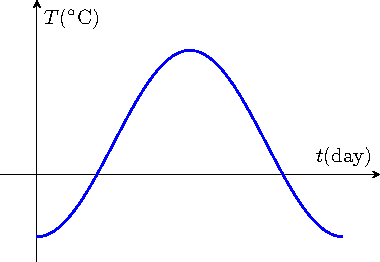
\includegraphics{fig-temperature_curve.pdf}
				\caption{Temperature curve}
				\label{fig:temp}
			\end{wrapfigure}
			
			We suppose that the temperature follows a sinusoidal curve, as shown in \textbf{Fig.\ref{fig:temp}}, as trigonometric functions are convenient for modeling periodical fluctuations.  We only consider locations in the northern hemisphere, so we further assume that the lowest temperature is reached on Jan.1st, or when $t = 0$.  We observe that the period of the function is 360 (for convenience, we suppose each month is 30 days long).  Thus, the equation for the curve is:
			
			\[
				T = -A \cos{\frac{2\pi}{360} t} + B.
			\]
			
			The points on this curve should satisfy the two following conditions:
			
			\[
				\mu_T = \frac1{360} \int_0^{360} (-A \cos{\frac{2\pi}{360} t} + B) \, \mathrm{d}t,
			\]
			
			\[
				\sigma_T^2 = \frac1{360} \int_0^{360} \left[ (-A \cos{\frac{2\pi}{360} t} + B) - \mu_T \right] ^2 	\mathrm{d}t.
			\]
			
			With the two equations above, we can solve for $A$ and $B$, and get
			
			\begin{equation} \label{eq:temp}
				T = -\sqrt2 \sigma_T \cos{\frac{2\pi}{360} t} + \mu_T.
			\end{equation}
	
	
	
		\subsubsection{Wind and Dispersal}
		\label{subsubsec:wind}
			
			For the direction of seed dispersal, we assume that the seed always follows the direction of the wind, which is uniformly distributed from 0$^\circ$ to 360$^\circ$ according to \textbf{Assumption \ref{assumption:wind}}.  
			
			For the distance of seed dispersal, we consider two types of wind, horizontal wind and updraft.  See \textbf{Fig.\ref{fig:dispersal}} for the two different types of wind.
			
			\begin{figure}[htbp]
				\centering
				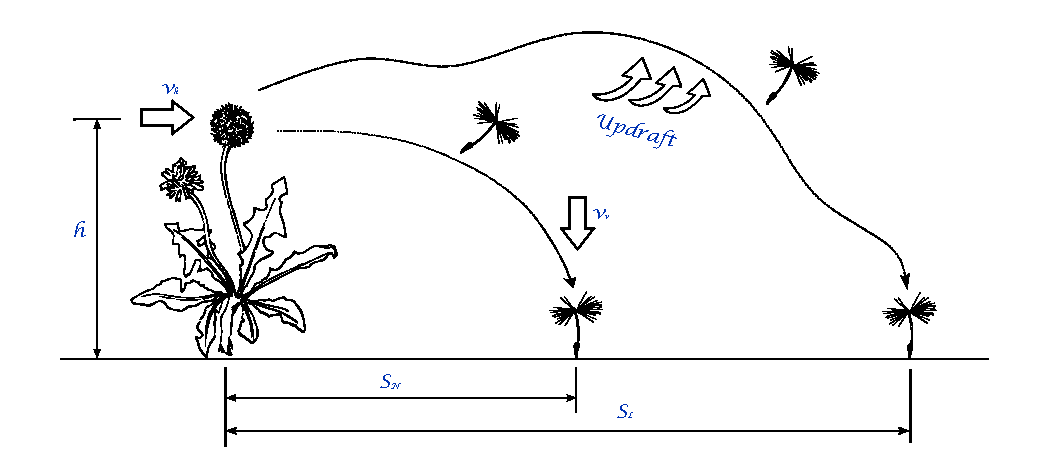
\includegraphics {wind_mode.pdf}
				\caption{Dandelion dispersal distance}
				\label{fig:dispersal}
			\end{figure}
			
			In the case of horizontal wind, we have
			\begin{equation}\label{eq:hwind}
				 \frac{s_N}{v_h} = \frac{h}{v_v},
			\end{equation}
			where $s_N$ ($N$ for \textit{N}ormal) is the distance that the seed travels, $v_h$ is the speed of the horizontal wind, $h$ is the height of the dandelion, and $v_v$ is the vertical component of the velocity of the seed.  $v_v$ follows a normal distribution with $\mu = \mu_W$ and $\sigma = \sigma_W$.  $h$ is known for any given plant.  $v_v$ is approximately constant, with value 0.4 m/s.  Thus, we can calculate the value of $s_N$.
			
			\begin{wrapfigure}{l}{0.579\textwidth}
				\centering
				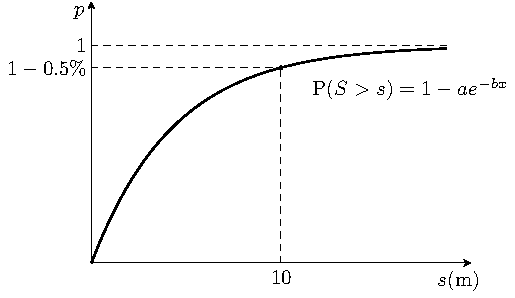
\includegraphics{fig-wind_curve.pdf}
				\caption{Cumulative distribution function of\\long-distance dispersal}
				\label{fig:longDistance}
			\end{wrapfigure}
			
			In the case of updraft, we suppose that the distance $s_L$ ($L$ for \textit{L}ong-distance) follows an exponential distribution, which can be expressed by the cumulative distribution function $\mathrm{P} (s_L < s) = 1 - ae^{-bs}$.  We know that $\mathrm{P} (s_L < 0) = 0$.  We also know that the probability of a seed being blown further than 10m is 0.5\%, i.e., $\mathrm{P} (s_L > 10) = 0.5\%$.  Therefore we can obtain
			
			\begin{equation}\label{eq:updraft}
				\mathrm{P} (s_L < s) = 1 - e^{-0.53 s}.
			\end{equation}
			
			We combine the two distances by taking $\max\{s_N, s_L\}$.   This is the distance that the seed travels.
			
			Finally, the leafs of dandelions have a radius of around 15cm.  If a seed were to land without falling on the leaf of another dandelion, the maximum density should be $(1/0.15)^2$ = 45 plants/m$^2$.  If a seed arrives at a location whose vicinity has a density greater than the maximum density, the seed fails to land.
		
		
		
		\subsubsection{Locations}
		
			We choose 6 locations in the US so that we have a variety of temperature and wind conditions.  Alaska is cold; California, the District of Columbia, and Kansas are warm; and Florida and Hawaii are relatively hot.  Alaska, the District of Columbia, and Kansas have distinct seasons; California and Florida show moderate temperature variation; and Hawaii has very stable temperature.  The wind conditions also exhibit different patterns.  The District of Columbia has notably large wind speed.
						
			{
				\fontsize{10}{14}\selectfont
				{
					\begin{longtable}{ccccccc}
						\caption{Environmental factors for six locations}
						\label{tb:locs}\\
						\toprule
						State&Abbreviation&$\mu_T$ ($^\circ$C)&$\sigma_T$ ($^\circ$C)&$\mu_W$ (m/s)&$\sigma_W$ (m/s)&$\mu_H$ (\%)\\
						\toprule
						Alaska&AK&-0.05&9.08&7.27&1.42&81.46\\
						California&CA&16.20&4.99&6.02&0.90&80.36\\
						District of Columbia&DC&12.64&8.63&13.97&9.51&77.49\\
						Florida&FL&22.11&4.76&6.51&1.71&77.05\\
						Hawaii&HI&22.75&1.40&6.23&0.69&74.64\\
						Kansas&KS&12.58&9.98&8.58&1.55&79.37\\
						\bottomrule
					\end{longtable}
				}
			}
		
		
		
		
		
	\subsection{Dandelion Life Cycle}
	
		We simulate the spread of dandelions by tracking every plant over time and recording its life stage and location.  A dandelion can transfer between 6 states, which are: \textbf{seed}, \textbf{developing}, \textbf{dispersal}, \textbf{inter-dispersal}, \textbf{hold}, and \textbf{dormancy}.  The previous four stages are shown in \textbf{Fig.\ref{fig:lifeCycle}}.
		
		\begin{figure}[htbp]
			\centering
			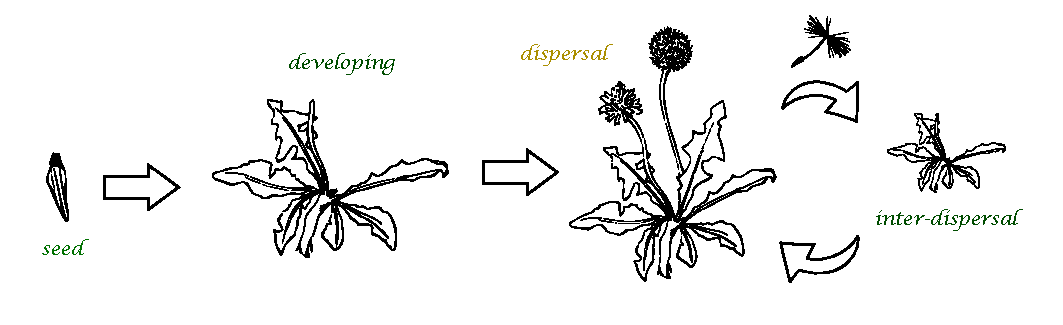
\includegraphics {life_cycle.pdf}
			\caption{Dandelion life cycle}
			\label{fig:lifeCycle}
		\end{figure}
		
		The duration of the developing stage, the height of the plant, and the number of seeds per head are determined by the adaption factor $k$.  The three parameters follow normal distributions with
		\begin{equation}\label{eq:k}
			\mu = \left( \mathrm{worst} + \frac{\mathrm{best} - \mathrm{worst}}4 \right) + k \frac{\mathrm{best} - \mathrm{worst}}2, \,
			\sigma = \frac{\mathrm{best} - \mathrm{worst}}{12}.
		\end{equation}
		The worst and best values for each of the parameters are given later in the section.
		
		Out of all the \textbf{seed}s that land in the field, only 2\% will successfully germinate.  These seeds will spend 3 days to grow into the developing stage.
		
		The \textbf{developing} stage lasts 69--107 days.  This is because it takes a seed 60--95 days to grow into a flower, and it takes an additional 9--12 days for the seeds on the flower to mature.  The exact duration of this stage is determined by $k$ (worst = 107, best = 69).  During this stage, the scape of the flower is grown.  The height of the flower is in the range 12--40cm and is determined by $k$ (worst = 12, best = 40).
		
		The \textbf{dispersal} stage lasts 10 days.  A dandelion plant can produce around 10 seed heads per year, and it usually flowers twice, so it produces 5 heads every time it blooms.  Each head has 150--200 seeds, and the exact number is determined by $k$ (worst = 150, best = 200).  It takes each head 2 days to disperse its seeds.  The seeds are dispersed per the method stated in \textbf{Section \ref{subsubsec:wind}}.
		
		When the temperature is higher than $24^\circ$C, only 12.5\% of the flowers bloom and disperse their seeds.  We let dandelions successfully enter the dispersal stage by a probability of 12.5\%, and the rest are moved into the hold stage.
		
		The \textbf{inter-dispersal} stage is the stage after dandelions exit dispersal and before they enter dispersal again.  In this stage, dandelions regrow their scapes and flowers.  Since most dandelions that flowered in spring usually flower again in fall, the duration of this stage is set to be exactly half a year, which is 180 days.  
		
		Dandelions can only enter the \textbf{hold} stage when $T > 24^\circ$C.  During this stage, flowers are held in buds and dispersal is diminished.  As soon as $T$ falls below $24^\circ$C, dandelions return to the stage before it entered the hold stage.  
		
		Dandelions can only enter the \textbf{dormancy} stage when $T < 0^\circ$C.  During this stage, the temperature is low and it is likely that it snows.  Therefore, all life activities of dandelions are paused.  As soon as $T$ rises above $0^\circ$C, dandelions resume the stage before it entered dormancy.
		
		
		
		
		
	\subsection{Algorithm}
	
	\subsection{Dandelion Spread Results}
	
		\subsubsection{Results}
		
			Our model contains several random variables.  We choose to use the Monte Carlo method to simulate.  We tally the number of dandelions and record the mean distance from (0, 0), the origin, where the first dandelion is located.
			
			First, we have to determine the starting time of simulation.  The model was run with the starting date set to Jan.\,1st, Feb.\,1st, \ldots, and Dec.\,1st for all 6 locations.  The results for Florida are shown in \textbf{Fig.\ref{fig:start}}.  We observe that the number varies greatly among the runs, but the mean distance is approximately the same.  For each location, the starting date is chosen such that the number of dandelions at the end of 12 months is maximized.  The number of dandelions corresponding to the chosen dates are marked blue in \textbf{Table \ref{tb:start}}.
			
			\begin{figure}[htbp]
				\centering
				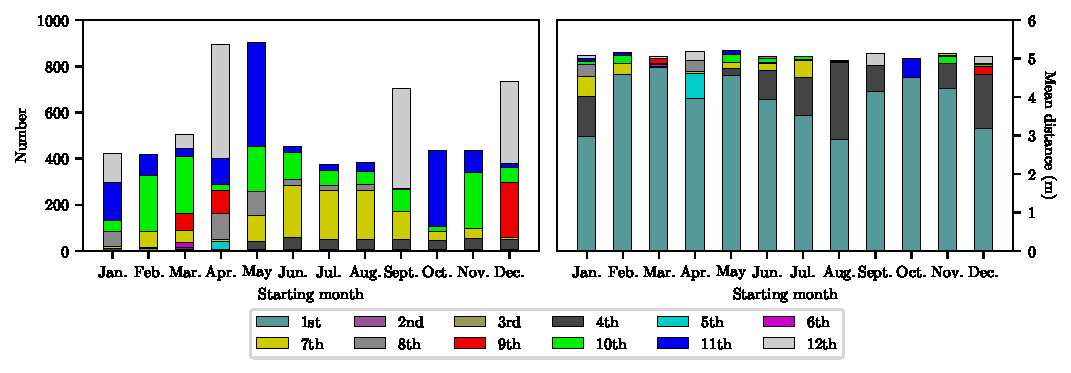
\includegraphics{start_month-number.pdf}
				\caption{Number and mean distance in Florida when simulation starts at different months}
				\label{fig:start}
			\end{figure}
			
			{
				\fontsize{10}{14}\selectfont
				{
					\begin{longtable}{ccccccccccccc}
						\caption{Number at six locations when simulation starts at different dates}
						\label{tb:start}\\
						\toprule
						State&Jan.&Feb.&Mar.&Apr.&May&Jun.&Jul.&Aug.&Sept.&Oct.&Nov.&Dec.\\
						\toprule
						AK&74&79&70&35&44&75&43&49&\color{blue}\textbf{82}&72&74&75\\
						CA&547&567&545&532&585&561&544&\color{blue}\textbf{596}&564&566&581&563\\
						DC&1611&1589&1609&1563&1680&1657&1673&1733&\color{blue}\textbf{1808}&1696&1677&1658\\
						FL&424&417&505&895&\color{blue}\textbf{905}&453&375&384&706&436&435&736\\
						HI&519&329&610&593&586&596&308&543&\color{blue}\textbf{618}&383&385&600\\
						KS&823&276&268&405&548&274&266&\color{blue}\textbf{1067}&287&288&950&834\\
						\bottomrule
					\end{longtable}
				}
			}
			
			Next we ran the model 1000 times for each location.  The resulting frequency histogram is shown in \textbf{Fig.\ref{fig:freqDand}}.  We can see that both the number and the mean distance follow a distribution similar to a normal one.  We calculated several statistics for each location, which are displayed in \textbf{Table \ref{tb:numDistribution}}.
			
			\begin{figure}[htbp]
				\centering
				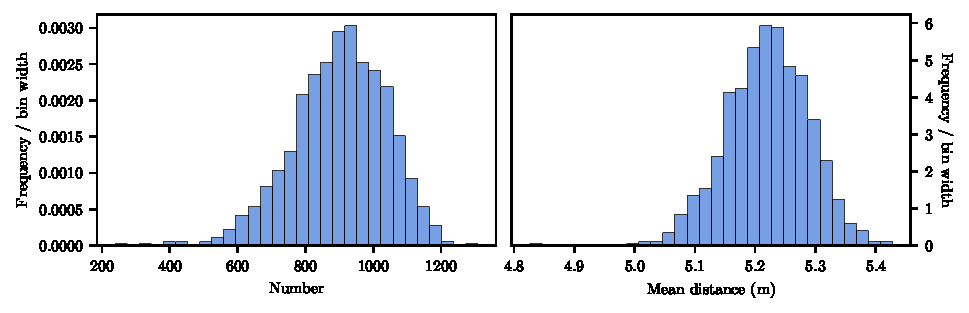
\includegraphics{number-frequency.pdf}
				\caption{Frequency distribution of number and mean distance in Florida}
				\label{fig:freqDand}
			\end{figure}
			
			We examine the distribution of the number of dandelions.  For all the locations, the confidence interval of the mean is relatively small, which implies the mean is quite accurate.  The standard deviation and range are relatively large, which shows that the spread of dandelions is easily affected by fluctuations in environmental factors and other random factors.  For all locations except California, the distribution is platykurtic, which means it is flatter and less concentrated than the normal distribution.  For all locations except Alaska, the distribution is skewed to the left.  The mass of the distribution is concentrated on the right, so the number of dandelions is slightly more likely to be greater than the mean rather than smaller.  However, because of the unfavorable environmental conditions in Alaska, the number is more likely to be smaller than the mean in that location.  We can draw the same conclusions from comparing the mean and the median as from the skewness.
			
			{
				\fontsize{10}{14}\selectfont
				{
					\begin{longtable}{cccccccc}
						\caption{Descriptive statistics of number at six locations}
						\label{tb:numDistribution}\\
						\toprule
						Location&Mean&Standard Deviation&Kurtosis&Skewness&Range&Median&Confidence Level (95.0\%)\\
						\toprule
						AK&72.7&26.5&-0.11&0.38&150&71&1.64\\
						CA&595.1&82.48&3.78&-1.32&744&609&5.11\\
						DC&1780&484.9&-0.04&-0.03&3274&1772.5&30.1\\
						FL&886.4&140.4&1.04&-0.72&981&905&8.71\\
						HI&607.5&81.9&1.12&-0.79&565&617&5.08\\
						KS&1066&186.4&1.05&-0.72&1403&1096&11.6\\
						\bottomrule
					\end{longtable}
				}
			}
			
			{
				\fontsize{10}{14}\selectfont
				{
					\begin{longtable}{cccccccc}
						\caption{Descriptive Statistics of the mean distance at six locations}
						\label{tb:distDistribution}\\
						\toprule
						Location&Mean&Standard Deviation&Kurtosis&Skewness&Range&Median&Confidence Level (95.0\%)\\
						\toprule
						AK&4.29&0.18&0.44&0.25&1.28&4.29&0.01\\
						CA&4.52&0.09&0.51&-0.53&0.67&4.52&0.01\\
						DC&11.84&0.21&1.5&-0.51&1.93&11.85&0.01\\
						FL&5.21&0.07&1.91&-0.64&0.66&5.21&0.00\\
						HI&4.99&0.08&0.138&-0.27&0.5&4.99&0.00\\
						KS&6.52&0.05&0.8&-0.36&0.44&6.52&0.00\\
						\bottomrule
					\end{longtable}
				}
			}
			
			Out of the 1000 runs, we selected the run that makes the number of dandelions closest to the mean value.  The positions and states of the dandelions at the end of 12 months are drawn in \textbf{Fig.\ref{fig:scatter5loc}}.  For all locations except the District of Columbia, most of the dandelions grow in a semicircular ring that is centered at the origin.  Alaska is apparently unsuitable for dandelions to spread.  In California, Hawaii, Florida, and Kansas, dandelions all spread at a moderate speed.
			
			\begin{figure}[htbp]
				\centering
				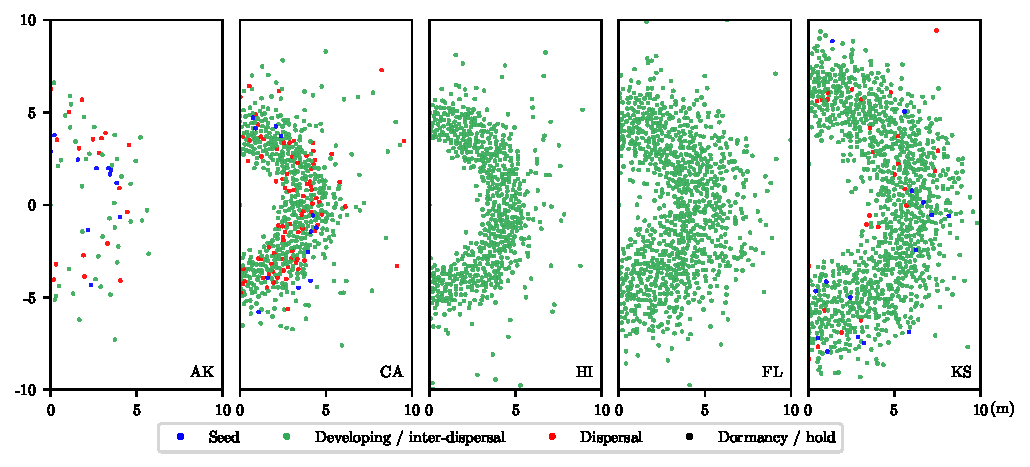
\includegraphics{spread_course-location_non_DC.pdf}
				\caption{The spread at the end of 12 months at different locations}
				\label{fig:scatter5loc}
			\end{figure}
			
			The positions and states of the dandelions at the end of each of the 12 months are plotted for the District of Columbia (see \textbf{Fig.\ref{fig:spreadDC}}).  The dandelions form a semicircle around the first dandelion.  The closer to the origin, the denser the plants.  Additionally, there is a burgeon every three months, which is caused by the flowering of a new generation of dandelions.
			
			\begin{figure}[htbp]
				\centering
				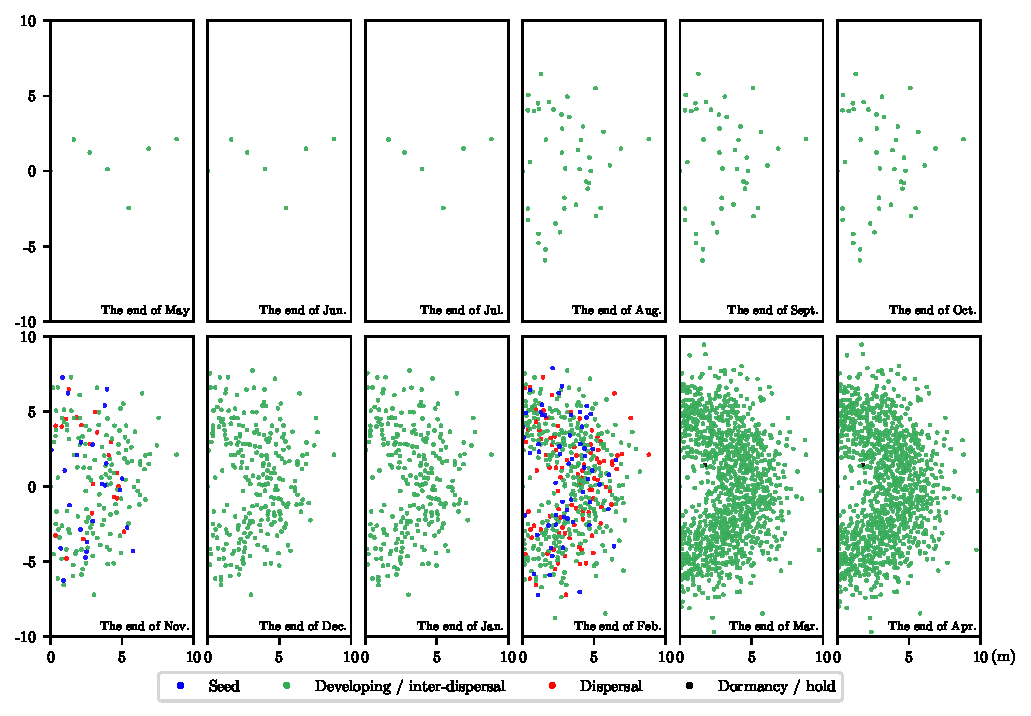
\includegraphics{spread_course-time.pdf}
				\caption{The spread during 12 months in the District of Columbia}
				\label{fig:spreadDC}
			\end{figure}
			
			Finally, we present a graph of the mean distance and natural logarithm of dandelion number in \textbf{Fig.\ref{fig:time}}.  The graph for ln(number) has several jumps and platforms.  The number has a periodic pattern and increases exponentially at the end of each period.  This conclusion coincides with our observation in \textbf{Fig.\ref{fig:spreadDC}}.  Again, Alaska is different because the dandelions are dormant in the first three months of the year.  
			
			\begin{figure}[htbp]
				\centering
				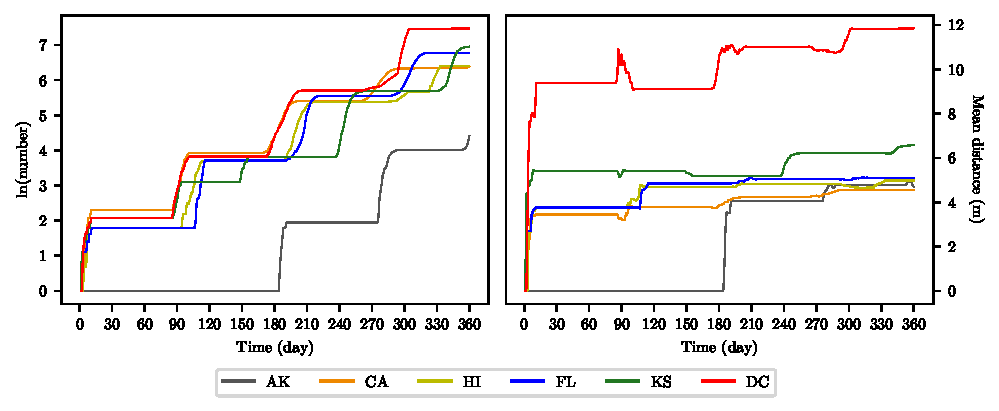
\includegraphics{number_mean_distance-time.pdf}
				\caption{Number and mean distance over time}
				\label{fig:time}
			\end{figure}
		
		
		
		\subsubsection{Sensitivity Analysis}
			
			We conduct a sensitivity analysis on the five factors by varying one of them while keeping the other four fixed.  
			
			\textbf{Fig.\ref{fig:saT}} shows the results for temperature.  When $\mu_T$ falls below 7$^\circ$C or rises above 23$^\circ$C, dandelion number decreases sharply.  This is because dandelions are transferred to the dormancy or hold stages at very low or very high temperatures.  Between these two temperatures there is a slow increase in number as $\mu_T$ increases.  The number is very sensitive to extreme temperatures, but only moderately responsive to mild temperatures.  The mean distance increases with $\mu_T$ up to 19$^\circ$C, where the it levels off and begins to fall at 23$^\circ$C.  It has medium sensitivity to $\mu_T$.
			
			Both number and mean distance decreases as $\sigma_T$ increases.  They decrease relatively slowly below $\sigma_T = 5^\circ$C and rapidly above that value.  However, the overall sensitivity is not high for either number or mean distance.
			
			\begin{figure}[htbp]
				\centering
				\begin{minipage}{0.04\textwidth}\end{minipage}
				\begin{minipage}{0.46\textwidth}
					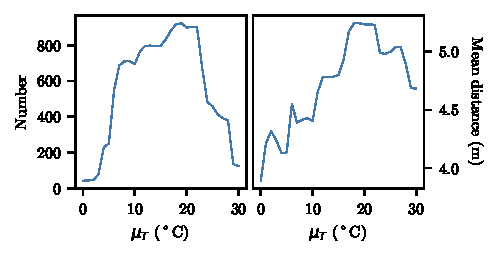
\includegraphics{sa_MuT.pdf}
				\end{minipage}
				\begin{minipage}{0.46\textwidth}
					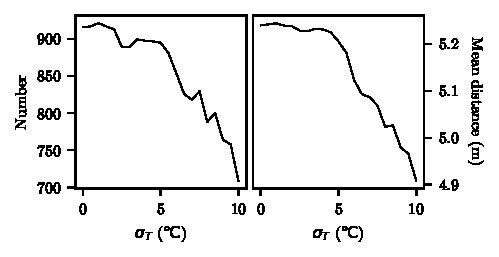
\includegraphics{sa_StdT.pdf}
				\end{minipage}
				\begin{minipage}{0.04\textwidth}\end{minipage}
				\caption{Sensitivity analysis: temperature}
				\label{fig:saT}
			\end{figure}
			
			\textbf{Fig.\ref{fig:saW}} shows the results for wind speed.  The number and mean distance have a positive correlation with $\mu_W$ and $\sigma_W$ and change drastically when the two factors vary.  When the mean wind speed increases, seeds are dispersed further apart from each other, so it is less likely for them to land on other plants.  When the standard deviation increases, some seeds land near the mother plant and others far.  
			
			\begin{figure}[htbp]
				\centering
				\begin{minipage}{0.04\textwidth}\end{minipage}
				\begin{minipage}{0.46\textwidth}
					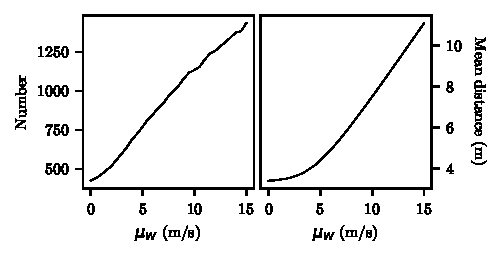
\includegraphics{sa_MuW.pdf}
				\end{minipage}
				\begin{minipage}{0.46\textwidth}
					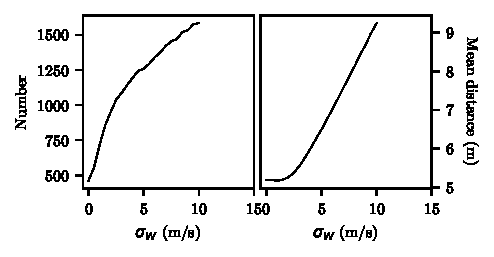
\includegraphics{sa_StdW.pdf}
				\end{minipage}
				\caption{Sensitivity analysis: wind speed}
				\label{fig:saW}
			\end{figure}
			
			\textbf{Fig.\ref{fig:saH}} shows the results for humidity.  
			
			\begin{figure}[htbp]
				\centering
				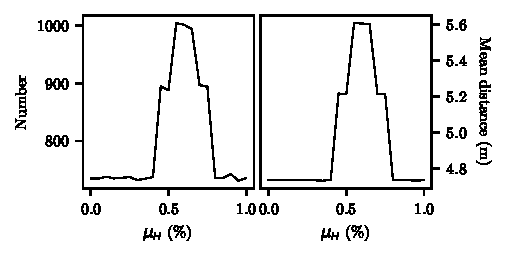
\includegraphics{sa_Hum.pdf}
				\caption{Sensitivity analysis: humidity}
				\label{fig:saH}
			\end{figure}
			
			
			
		\subsubsection{Strengths and Weaknesses}
		
		

		
		
		
		
\section{Plant Impact Factor Model}

	\subsection{Assumptions and Justifications}
	
	\subsection{Model Description}

		hello
		
		{
			\fontsize{10}{14}\selectfont
			{
			\begin{longtable}{p{0.2in}p{1.5in}p{4.3in}}
				
				\caption{Attributes}
				\label{tb:attributes}\\
				
				\toprule
				\multicolumn{1}{c}{\textbf{Symbol}} 
					& \multicolumn{1}{c}{\textbf{Attributes}}
					& \multicolumn{1}{c}{\textbf{$a_i$, $b_i$ and $c_i$ Evaluation}} \\
			
				\toprule
				\multicolumn{3}{l}{Category $A$ - Plant Characteristics}\\
				\midrule
				
				$A_1$ & Duration & $a_1=0.5$ (Annual), $0.75$ (Biennial), $1$ (Perennial)\\
				$A_2$ & Growing Habit & $a_2=0$ (Tree), $0.25$ (Shrub), $0.5$ (Vine), $0.75$ (Graminoid), $1$ (Forb/herb)\\ 
				$A_3$ & Growth Rate & The growth rate after successful establishment\\
					&& $a_3=0.5$ (Slow), $0.75$ (Moderate), $1$ (Rapid)\\
				$A_4$ & Lifespan & $a_4=0.25$ (when $a_1=0.5$ or $0.75$), $0.5$ (Short), $0.75$ (Moderate), $1$ (Long) \\
				$A_5$ & Fertility Requirement & Relative level of nutrition (N, P, K) required for normal growth and development.\\
					 && $a_5=0.5$ (Low), $0.75$ (Medium), $1$ (High)\\
				$A_6$ & Fruit/Seed Abundance & The amount of seed produced.\\
					&& $a_6=0.25$ (None), $0.5$ (Low), $0.75$ (Medium), $1$ (High)\\
				$A_7$ & Propagated Methods & The propagetion methods number, $n_7$. The methods can be Propagated by Bare Root, by Bulb, by Container, by Corm, by Cuttings, by Seed, by Sod, by Sprigs, or by Tubers. \\
					&& $a_7=0.25$ ($n_7=1$), $0.5$ ($n_7=2$), $0.75$ ($n_7=3$), $1$ ($n_7\geq4$)\\
				$A_8$ & Seed Spread Rate & The capability of the plant to spread through its seed production.\\
					&& $a_8=0.25$ (None), $0.5$ (Slow), $0.75$ (Moderate), $1$ (Rapid)\\
				$A_9$ & Seedling Vigor & The expected seedling survival percentage of the plant\\
					&& $a_9=0.5$ (Low), $0.75$ (Medium), $1$ (High)\\
				
				\midrule
				\multicolumn{3}{l}{Category $B$ - Human and Environment}  \\
				\midrule
				
				$B_1$ & Toxicity & The relative toxicity of the plant to either humans or livestock.\\
					&& $b_1=0$ (None), $0.5$ (Slight), $0.75$ (Moderate), $1$ (Severe)\\
				$B_2$ & Product & The level of the plant known to be suitable for multiple types of products.\\
					&& $b_2=0$ (Copiousness), $0.25$ (Many), $0.5$ (Some), $0.75$ (few), $1$ (None)\\
				$B_3$ & Palatable Animal & The relative palatability of this plant to browsing animals or to grazing animals.\\
					&& $b_3=0$ (High), $0.5$ (Moderate), $0.75$ (Low), $1$ (None)\\
				$B_4$ & Palatable Human & The plant produce berries, nuts, seeds, or fruits are palatable to humans. \\
					&& $b_4=0.5$ (Yes), $1$ (No)\\
				$B_5$ & Commercial Availability & The plant propagules are in the commercial marketplace \\
					&& $b_5=0.5$ (Yes), $1$ (No)\\
			
				\midrule
				\multicolumn{3}{l}{Category $C$ - Location}  \\
				\midrule
				
				$C_1$ & Soil Adaption & The soil adaption level\\
				&& $c_1=0$ (Low), $0.5$ (Medium), $1$ (High)\\
				$C_2$ & Temperature Adaption & The temperature adaption level\\
				&& $c_2=0$ (Low), $0.5$ (Medium), $1$ (High)\\
				$C_3$ & Humid Adaption & The humid adaption level\\
				&& $c_3=0$ (Low), $0.5$ (Medium), $1$ (High)\\
				$C_4$ & Population Density & The level of population density.\\
				&& $c_4=0$ (High), $0.5$ (Medium), $1$ (Low)\\
			
				\bottomrule
			
			\end{longtable}
			}
		}
		
		{
			\fontsize{10}{18}\selectfont
			{
				\begin{longtable}{c|ccccccccc|ccccc||cccc}
					
					\caption{AHP comparison matrix}
					\label{tb:mat}\\
					
					\toprule
					&$A_1$&$A_2$&$A_3$&$A_4$&$A_5$&$A_6$&$A_7$&$A_8$&$A_9$&$B_1$&$B_2$&$B_3$&$B_4$&$B_5$&$C_1$&$C_2$&$C_3$&$C_4$\\
					\toprule
					$A_1$&$1$&$1/3$&$1/7$&$1/3$&$1$&$1/7$&$1/4$&$1/7$&$1/5$&$1/9$&$1/5$&$1/3$&$1/4$&$1/4$&$1/5$&$1/5$&$1/5$&$1/3$\\
					$A_2$&$3$&$1$&$1/5$&$1$&$3$&$1/5$&$1/2$&$1/5$&$1/3$&$1/7$&$1/3$&$1$&$1/2$&$1/2$&$1/3$&$1/3$&$1/3$&$1$\\
					$A_3$&$7$&$5$&$1$&$5$&$7$&$1$&$4$&$1$&$3$&$1/3$&$3$&$5$&$4$&$4$&$3$&$3$&$3$&$5$\\
					$A_4$&$3$&$1$&$1/5$&$1$&$3$&$1/5$&$1/2$&$1/5$&$1/3$&$1/7$&$1/3$&$1$&$1/2$&$1/2$&$1/3$&$1/3$&$1/3$&$1$\\
					$A_5$&$1$&$1/3$&$1/7$&$1/3$&$1$&$1/7$&$1/4$&$1/7$&$1/5$&$1/9$&$1/5$&$1/3$&$1/4$&$1/4$&$1/5$&$1/5$&$1/5$&$1/3$\\
					$A_6$&$7$&$5$&$1$&$5$&$7$&$1$&$4$&$1$&$3$&$1/3$&$3$&$5$&$4$&$4$&$3$&$3$&$3$&$5$\\
					$A_7$&$4$&$2$&$1/4$&$2$&$4$&$1/4$&$1$&$1/4$&$1/2$&$1/4$&$1/2$&$2$&$1$&$1$&$1/2$&$1/2$&$1/2$&$2$\\
					$A_8$&$7$&$5$&$1$&$5$&$7$&$1$&$4$&$1$&$3$&$1/3$&$3$&$5$&$4$&$4$&$3$&$3$&$3$&$5$\\
					$A_9$&$5$&$3$&$1/3$&$3$&$5$&$1/3$&$2$&$1/3$&$1$&$1/5$&$1$&$3$&$2$&$2$&$1$&$1$&$1$&$3$\\
					\midrule
					$B_1$&$9$&$7$&$3$&$7$&$7$&$3$&$4$&$3$&$5$&$1$&$5$&$7$&$4$&$4$&$5$&$5$&$5$&$7$\\
					$B_2$&$5$&$3$&$1/3$&$3$&$5$&$1/3$&$2$&$1/3$&$1$&$1/5$&$1$&$3$&$2$&$2$&$1$&$1$&$1$&$3$\\
					$B_3$&$3$&$1$&$1/5$&$1$&$3$&$1/5$&$1/2$&$1/5$&$1/3$&$1/7$&$1/3$&$1$&$1/2$&$1/2$&$1/3$&$1/3$&$1/3$&$1$\\
					$B_4$&$4$&$2$&$1/4$&$2$&$4$&$1/4$&$1$&$1/4$&$1/2$&$1/4$&$1/2$&$2$&$1$&$1$&$1/2$&$1/2$&$1/2$&$2$\\
					$B_5$&$4$&$2$&$1/4$&$2$&$4$&$1/4$&$1$&$1/4$&$1/2$&$1/4$&$1/2$&$2$&$1$&$1$&$1/2$&$1/2$&$1/2$&$2$\\
					\midrule
					\midrule
					$C_1$&$5$&$3$&$1/3$&$3$&$5$&$1/3$&$2$&$1/3$&$1$&$1/5$&$1$&$3$&$2$&$2$&$1$&$1$&$1$&$3$\\
					$C_2$&$5$&$3$&$1/3$&$3$&$5$&$1/3$&$2$&$1/3$&$1$&$1/5$&$1$&$3$&$2$&$2$&$1$&$1$&$1$&$3$\\
					$C_3$&$5$&$3$&$1/3$&$3$&$5$&$1/3$&$2$&$1/3$&$1$&$1/5$&$1$&$3$&$2$&$2$&$1$&$1$&$1$&$3$\\
					$C_4$&$3$&$1$&$1/5$&$1$&$3$&$1/5$&$1/2$&$1/5$&$1/3$&$1/7$&$1/3$&$1$&$1/2$&$1/2$&$1/3$&$1/3$&$1/3$&$1$\\
					\bottomrule
				\end{longtable}
			}
		}	

		hello!!! \\

		{
			\fontsize{10}{14}\selectfont
			{
				\begin{longtable}{cccccccc}
					\caption{Consistency test}
					\label{tb:consistency}\\
					
					\toprule
					Impact Factor&Attribute Number&max eigenvalue 
					&\multirow{2}{*}{$\mathrm{CI}=\frac{\lambda_{max}-n}{n-1}$}
					&\multirow{2}{*}{$\mathrm{RI}$}
					&\multirow{2}{*}{$\mathrm{CR}=\frac{\mathrm{CI}}{\mathrm{RI}}$}
					&\multirow{2}{*}{$\mathrm{CR}<0.1?$}\\
					Type&$n$&$\lambda_{max}$\\
					\toprule
					Global&$14$&$14.501$&$0.0386$&$1.49$&0.0259&Yes\\
					Local&$18$&$18.561$&$0.0330$&$1.49$&0.0221&Yes\\
					\bottomrule
				\end{longtable}
			}
		}	

	hello!!! \\
	hello!!! \\
	hello!!! \\
	hello!!! \\
	
		{
			\fontsize{10}{14}\selectfont
			{
				\begin{longtable}{c|ccccccccc}
					\caption{Weights results}
					\label{tb:weights}\\
					
					\toprule
					Type&$\alpha_1$&$\alpha_2$&$\alpha_3$&$\alpha_4$&$\alpha_5$&$\alpha_6$&$\alpha_7$&$\alpha_8$&$\alpha_9$\\
					\toprule
					Global&0.014&0.027&0.134&0.027&0.014&0.134&0.044&0.134&0.066\\
					Local&0.011&0.021&0.113&0.021&0.011&0.113&0.034&0.113&0.052\\
					\toprule
					\toprule
					&$\beta_1$&$\beta_2$&$\beta_3$&$\beta_4$&$\beta_5$&$\gamma_1$&$\gamma_2$&$\gamma_3$&$\gamma_4$\\
					\toprule
					Global&0.227&0.066&0.027&0.044&0.044&-&-&-&-\\
					Local&0.192&0.052&0.021&0.034&0.034&0.052&0.052&0.052&0.021\\
					\bottomrule
				\end{longtable}
			}
		}	
	
		hello!!! \\
		
		{
			\fontsize{10}{14}\selectfont
			{
				\begin{longtable}{cccccc}
					\caption{Plant Rankings}
					\label{tb:ranks}\\
					
					\toprule
					Rank&Scientific Name&Vernacular Name&Duration&Growing Habit&IF$_g$\\
					\toprule
					1&Melilotus officinalis&Sweetclover&Perennial&Forb/herb&84.5\\
					2&Senecio vulgaris&Old-man-in-the-spring&Biennial&Forb/herb&83.3\\
					3&Ailanthus altissima&Tree of heaven&Perennial&Tree&81.8\\
					4&Crotalaria spectabilis&Showy rattlebox&Annual&Forb/herb&81.7\\
					5&Ranunculus repens&Creeping buttercup&Perennial&Forb/herb&80.8\\
					6&Melilotus indicus&Annual yellow sweetclover&Annual&Forb/herb&80.0\\
					7&Digitalis purpurea&Purple foxglove&Biennial&Forb/herb&79.9\\
					8&Sorghum halepense&Johnsongrass&Perennial&Graminoid&78.9\\
					9&Schedonorus arundinaceus&Tall fescue&Perennial&Graminoid&76.8\\
					10&Vicia sativa&Garden vetch&Annual&Forb/herb&73.8\\
					$\vdots$\\
					26&Taraxacum officinale&Common dandelion&Perennial&Forb/herb&66.9\\
					\bottomrule
				\end{longtable}
			}
		}
		
		remember to write the sample quantity and unit \\

		{
			\fontsize{10}{14}\selectfont
			{
				\begin{longtable}{ccccccc}
					\caption{Distribution of impact factor}
					\label{tb:IFDistribution}\\
					
					\toprule
					Mean&Standard Deviation&Kurtosis&Skewness&Range&Median&Confidence Level (95.0\%)\\
					\toprule
					57.9&8.65&0.81&0.41&50.51&57.25&1.13\\
					\bottomrule
				\end{longtable}
			}
		}
		
		hello!!! \\

		{
			\fontsize{10}{14}\selectfont
			{
				\begin{longtable}{p{6.5in}}
					\toprule
					\fontsize{12}{18}\selectfont{\textbf{Algorithm 1} Monte Carlo simulation algorithm for dandelion spread}\\
					\toprule
					\textbf{INPUT:} run times \toB{$n$ } and environment factors \toB{$\mu_T$}, \toB{$\sigma_T$}, \toB{$\mu_W$}, \toB{$\sigma_W$ } and \toB{$\mu_H$}\\
					\textbf{OUTPUT:} dandelion spread \toB{$numbers$} and mean \toB{$distances$ } over days\\
					\textbf{Begin Procedure}
					\begin{algorithmic}
						\For{1 to \toB{$n$}}
						\ForAll{\toB{$t$ } in days of one year}
						\For{\toB{$dandelion$ } in current all dandelions}
						\State \toB{$T$ } $\gets$ evaluate current temperature per \textbf{Equation} \ref{eq:temp}
						\State \toB{$T$ } $\gets$ evaluate current temperature per \textbf{Equation} \ref{eq:temp}
						\EndFor
						\EndFor
						\EndFor
						\State \textbf{Return}{ \toB{$numbers$ } and \toB{$distances$}}
					\end{algorithmic}
					\textbf{End Procedure}\\
					\bottomrule
				\end{longtable}
			}
		}
		
		hello!!! \\

	\subsection{Sensitivity Analysis}
	
		\begin{figure}[htbp]
			\centering
			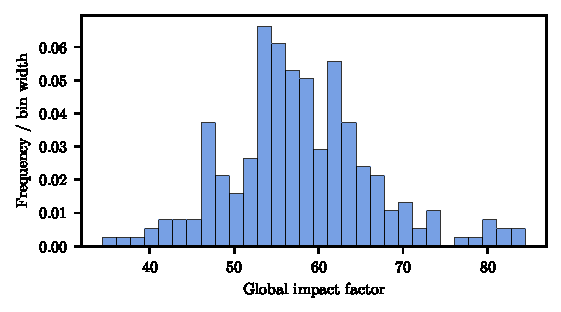
\includegraphics{IF-frequency.pdf}
			\caption{Frequency distribution of global impact factor}
			\label{fig:freqIF}
		\end{figure}
	
		\begin{figure}[htbp]
			\centering
			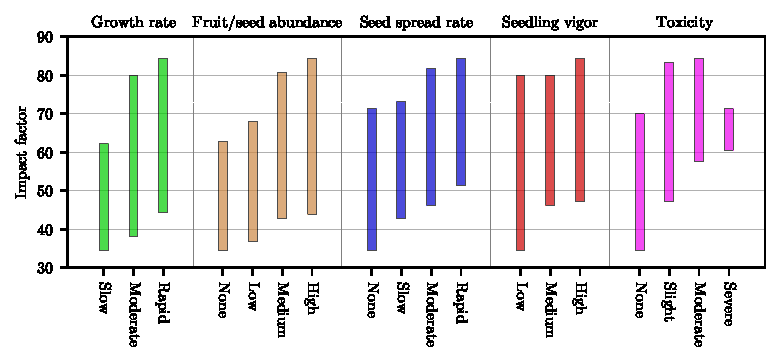
\includegraphics{categories-IF.pdf}
			\caption{Sensitivity analysis}
			\label{fig:IFfactors}
		\end{figure}
		
		\begin{figure}[htbp]
			\centering
			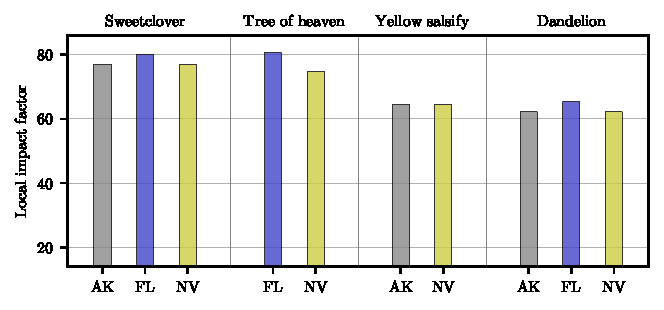
\includegraphics{IF_local-loc.pdf}
			\caption{Local impact factor}
			\label{fig:IFLocal}
		\end{figure}
		
	\subsection{Strengths and Weaknesses}

		some random text
	
\section*{We Share the Earth}
\addcontentsline{toc}{section}{We Share the Earth}



\newrefcontext
\printbibliography

\end{document}
